\documentclass[11pt,reqno]{amsart}

\usepackage{amsmath,amsthm,amssymb,comment,fullpage}
%\usepackage{epsf, subfigure, verbatim}
\usepackage{braket}
\usepackage{mathtools}

%\usepackage{euler,palatino}
%\usepackage{srcltx}
%\usepackage{amsthm}
%\usepackage[latin1]{inputenc}
%\usepackage[T1]{fontenc}
%\usepackage{float}

%\usepackage{mathrsfs}
%\documentclass[12pt,reqno]{amsart}
\usepackage{caption}
\usepackage{subcaption}
\usepackage{times}
\usepackage[T1]{fontenc}
\usepackage{mathrsfs}
\usepackage{latexsym}
\usepackage[dvips]{graphics}
\usepackage{epsfig}
%\usepackage{hyperref, amsmath, amsthm, amsfonts, amscd, flafter,epsf}
\usepackage{amsmath,amsfonts,amsthm,amssymb,amscd}
\input amssym.def
\input amssym.tex
\usepackage{color}
\usepackage{hyperref}
\usepackage{url}
%\usepackage{breakurl}
\newcommand{\bburl}[1]{\textcolor{blue}{\url{#1}}}

\usepackage{tikz}
\usepackage{tkz-tab}
\usepackage{tkz-graph}
\usetikzlibrary{shapes.geometric,positioning}
%\newcommand{\burl}[1]{\textcolor{blue}{\url{#1}}}
\newcommand{\blue}[1]{\textcolor{blue}{(\bf{#1})}}


%\usepackage{showkeys}
%\DeclareGraphicsRule{.tif}{png}{.png}{`convert #1 `dirname #1`/`basename #1 .tif`.png}

\newcommand{\emaillink}[1]{\textcolor{blue}{\href{mailto:#1}{#1}}}

\newcommand{\burl}[1]{\textcolor{blue}{\url{#1}}}
\newcommand{\fix}[1]{\textcolor{red}{\textbf{ (#1)\normalsize}}}
\newcommand{\fixed}[1]{\textcolor{green}{~\\ \textbf{#1\normalsize}}\\}

\newcommand{\ind}{\otimes}
\newcommand{\witi}{\widetilde}
\newcommand{\dt}[1]{\witi{\witi #1}}
\newcommand{\ol}[1]{\overline{#1}}
\newcommand{\lr}[1]{\left\lfloor#1\right\rfloor}
\newcommand{\eqd}{\overset{\footnotesize{d}}{=}}
\newcommand{\calf}{{\mathcal F}}
\newcommand{\cal}{\mathcal}

\renewcommand{\theequation}{\thesection.\arabic{equation}}
\numberwithin{equation}{section}


\newtheorem{thm}{Theorem}[section]
\newtheorem{conj}[thm]{Conjecture}
\newtheorem{cor}[thm]{Corollary}
\newtheorem{lem}[thm]{Lemma}
\newtheorem{prop}[thm]{Proposition}
\newtheorem{exa}[thm]{Example}
\newtheorem{defi}[thm]{Definition}
\newtheorem{exe}[thm]{Exercise}
\newtheorem{que}[thm]{Question}
\newtheorem{prob}[thm]{Problem}
\newtheorem{cla}[thm]{Claim}
\newtheorem{proj}[thm]{Research Project}

\theoremstyle{plain}
\newtheorem{X}{X}[section]
\newtheorem{corollary}[thm]{Corollary}
\newtheorem{definition}[thm]{Definition}
\newtheorem{example}[thm]{Example}
\newtheorem{lemma}[thm]{Lemma}
\newtheorem{proposition}[thm]{Proposition}
\newtheorem{theorem}[thm]{Theorem}
\newtheorem{problem}[thm]{Problem}
\newtheorem{conjecture}[thm]{Conjecture}
\newtheorem{hypothesis}[thm]{Hypothesis}
\newtheorem{remark}[thm]{Remark}
%\newtheorem*{hyptheta}[thm]{Hypothesis \ref{montgomery original}$_\theta$}
%\newtheorem*{hyplog}{Hypothesis \ref{montgomer original}}
%\newtheorem*{hypsmallo}[thm]{Hypothesis \ref{montgomery original}}
%\newtheorem*{hypeta}[thm]{Hypothesis 1.10$_{\eta}$}


%\theoremstyle{definition}

\renewcommand\thesection{\arabic{section}}
\newcommand{\F}{\mathscr{F}}
\newcommand{\f}{\widehat{\eta}}


%%%%%%%%%%%%%% Dirichlet characters
\newcommand{\Norm}[1]{\frac{#1}{\sqrt{N}}}

\newcommand{\sumii}[1]{\sum_{#1 = -\infty}^\infty}
\newcommand{\sumzi}[1]{\sum_{#1 = 0}^\infty}
\newcommand{\sumoi}[1]{\sum_{#1 = 1}^\infty}

\newcommand{\eprod}[1]{\prod_p \left(#1\right)^{-1}}
%$(s,b)$-Generacci
\newcommand{\sbg}{(s,b)\text{-Generacci}}
\newcommand{\sbs}{(s,b)\text{-Generacci\ sequence}}
\newcommand{\fqs}{\text{Fibonacci\ Quilt\ sequence}}
\newcommand{\fq}{\text{Fibonacci\ Quilt}}
\newcommand\st{\text{s.t.\ }}
\newcommand\be{\begin{equation}}
\newcommand\ee{\end{equation}}
\newcommand\bee{\begin{equation*}}
\newcommand\eee{\end{equation*}}
\newcommand\bea{\begin{eqnarray}}
\newcommand\eea{\end{eqnarray}}
\newcommand\beae{\begin{eqnarray*}}
\newcommand\eeae{\end{eqnarray*}}
\newcommand\bi{\begin{itemize}}
\newcommand\ei{\end{itemize}}
\newcommand\ben{\begin{enumerate}}
\newcommand\een{\end{enumerate}}
\newcommand\bc{\begin{center}}
\newcommand\ec{\end{center}}
\newcommand\ba{\begin{array}}
\newcommand\ea{\end{array}}
%\newcommand\mod{\text{mod\ }}
\newcommand{\mo}{\text{mod}\ }

\newcommand\ie{{i.e.,\ }}
\newcommand{\tbf}[1]{\textbf{#1}}
\newcommand\CF{{Continued Fraction}}
\newcommand\cf{{continued fraction}}
\newcommand\cfs{{continued fractions}}
\newcommand\usb[2]{\underset{#1}{\underbrace{#2}}}


%kmin and kmax
\newcommand{\kmin}[1]{k_{\min}(#1)}
\newcommand{\kmax}[1]{k_{\max}(#1)}
\newcommand{\kminm}{K_{\min}(m)}
\newcommand{\kmaxm}{K_{\max}(m)}
\newcommand{\B}{\mathcal{B}}
% General Symbols

\def\notdiv{\ \mathbin{\mkern-8mu|\!\!\!\smallsetminus}}
\newcommand{\done}{\Box} %use in linux
%\newcommand{\umess}[2]{\underset{(#1)}{\underbrace{#2}}}
\newcommand{\umessclean}[2]{\underset{=#1}{\underbrace{#2}}}

%Blackboard Letters

\newcommand{\R}{\ensuremath{\mathbb{R}}}
\newcommand{\C}{\ensuremath{\mathbb{C}}}
\newcommand{\Z}{\ensuremath{\mathbb{Z}}}
\newcommand{\Q}{\mathbb{Q}}
\newcommand{\N}{\mathbb{N}}
%\newcommand{\F}{\mathbb{F}}
\newcommand{\W}{\mathbb{W}}
\newcommand{\Qoft}{\mathbb{Q}(t)}  %use in linux

\newcommand\frakfamily{\usefont{U}{yfrak}{m}{n}}
\DeclareTextFontCommand{\textfrak}{\frakfamily}
\newcommand\G{\textfrak{G}}


% Fractions

\newcommand{\fof}{\frac{1}{4}}  %oneforth
\newcommand{\foh}{\frac{1}{2}}  %onehalf
\newcommand{\fot}{\frac{1}{3}}  %onethird
\newcommand{\fop}{\frac{1}{\pi}}    %1/pi
\newcommand{\ftp}{\frac{2}{\pi}}    %2/pi
\newcommand{\fotp}{\frac{1}{2 \pi}} %1/2pi
\newcommand{\fotpi}{\frac{1}{2 \pi i}}
\newcommand{\cm}{c_{\text{{\rm mean}}}}
\newcommand{\cv}{c_{\text{{\rm variance}}}}

% Theorem / Lemmas et cetera

%\theoremstyle{definition}

\newcommand{\vars}[2]{ #1_1, \dots, #1_{#2} }
\newcommand{\ncr}[2]{{#1 \choose #2}}
\newcommand{\twocase}[5]{#1 \begin{cases} #2 & \text{{\rm #3}}\\ #4
&\text{{\rm #5}} \end{cases}   }
\newcommand{\threecase}[7]{#1 \begin{cases} #2 & \text{{\rm #3}}\\ #4
&\text{{\rm #5}}\\ #6 & \texttt{{\rm #7}} \end{cases}   }
\newcommand{\twocaseother}[3]{#1 \begin{cases} #2 & \text{#3}\\ 0
&\text{otherwise} \end{cases}   }


%Formatting
\renewcommand{\baselinestretch}{1}
\newcommand{\murl}[1]{\href{mailto:#1}{\textcolor{blue}{#1}}}
\newcommand{\hr}[1]{\href{#1}{\url{#1}}}

%%% NEW COMMANDS FOR THIS PAPER
\newcommand{\dfq}{d_{\rm FQ}}
\newcommand{\dave}{d_{\rm FQ; ave}}
\newcommand{\daven}{d_{\rm FQ; ave}(n)}
\newcommand{\todo}[1]{\textcolor{red}{\textbf{#1}}}
\newcommand{\DN}[1]{\textcolor{blue}{\textbf{(DN:#1)}}}
\newcommand{\PF}[1]{\textcolor{cyan}{\textbf{(PF:#1)}}}
\newcommand{\ch}{\textnormal{ch}}
\newcommand{\textAnd}{\hspace{3mm}\textnormal{and}\hspace{3mm}}


%%% NEW COMMANDS FROM VARIANCE
\newcommand{\PP}[1]{\mathbb{P}[#1]}
\newcommand{\E}[1]{\mathbb{E}[#1]}
\newcommand{\V}[1]{\text{{\rm Var}}[#1]}
\newcommand{\BS}{\mathcal{S}}
\newcommand{\T}{\mathcal{T}}
\newcommand{\LT}{\mathcal{L_T}}
\newcommand{\LS}{\mathcal{L_S}}
\newcommand{\ZS}{\mathcal{Z_S}}
\newcommand{\ds}{\displaystyle}
\newcommand{\nsum}{Y_n}


\def\twobytwoMat(#1, #2, #3, #4){
    {
        \begin{bmatrix}
            {#1} & {#2}\\
            {#3} & {#4}
        \end{bmatrix}
    }
}

\def\twobyoneMat(#1, #2){
    {
        \begin{bmatrix}
            {#1}\\
            {#2}
        \end{bmatrix}
    }
}

\def\twobytwoDet(#1, #2, #3, #4){
    {
        \begin{vmatrix}
            {#1} & {#2}
            {#3} & {#4}
        \end{vmatrix}
    }
}


\newcommand\blfootnote[1]{%
  \begingroup
  \renewcommand\thefootnote{}\footnote{#1}%
  \addtocounter{footnote}{-1}%
  \endgroup
}



\title{Analysis on Leslie Population Models: Predator-Prey Model, Competetive Model, and the Migration Model}

\author[Miller, Son, Wang]{Steven J. Miller, Daniel Son, Janine Wang}

% \author{Your Name}
% \email{\textcolor{blue}{\href{mailto:youremail@school.edu}{youremail@school.edu}}}
% \address{Department of Mathematics, School, City, Zip}


% \author{Steven J. Miller}
% \email{\textcolor{blue}{\href{mailto:sjm1@williams.edu}{sjm1@williams.edu}},  \textcolor{blue}{\href{Steven.Miller.MC.96@aya.yale.edu}{Steven.Miller.MC.96@aya.yale.edu}}}
% \address{Department of Mathematics and Statistics, Williams College, Williamstown, MA 01267}

% \author{Daeyoung Son}
% \email{\textcolor{blue}{\href{mailto:ds15@williams.edu}{ds15@williams.edu}}}
% \address{Department of Mathematics and Statistics, Williams College, Williamstown, MA 01267}

% \author{Janine Wang}
% \email{\textcolor{blue}{\href{mailto:jjw3@williams.edu}{jjw3@williams.edu}}}



\thanks{Miller was partially supported by NSF grant DMS1265673. We thank....}

\subjclass[2010]{60B10, 11B39, 11B05  (primary) 65Q30 (secondary)}

\keywords{Predator-Prey Model, Leslie Matrix, Migration Model, Quantum Operators}

\date{\today}


\begin{document}

\blfootnote{
\begin{center}
\textit{Email addresses:}\texttt{~sjm1@williams.edu} (Steven J. Miller),\texttt{~ds15@williams.edu} (Daeyoung Son),\texttt{~jjw3@williams.edu} (Janine Wang)
\end{center}
}
\maketitle


\begin{abstract} 

    
In this paper, we introduce a new predator-prey model based 
the Lotka-Voltera model. Extensive study have been conducted 
on the stability of the equation for the simple model which 
considers an homogenous population
. For example, Merdan \cite{Merdan2009} 
\cite{Merdan2010} carries 
out a stability analysis by computing the Jacobian and 
drawing from methods of differential calculus and Zhou \cite{Zhou2005} studied different types of Allee effects and 
the corresponding stability. 

We replace the population evolution constants 
to a Leslie matrix, taking account of multiple age groups. 
Replacing the constant coefficients to 
Leslie matrices motivates the study of dominant eigenvalues 
which can be conducted using techniques in Complex Analysis. 
Using the theory of dominating eigenvalues, we provide a bound 
for maximum predation rate for population survival in a long term. 
We also discuss the competitive model, and prove the 
last species standing theorem, which describes the unlikelihood 
of stable equilibrium between two competitive species. 

Moreover, we analyze an open population where migration 
is allowed. We first study 
population under constant migration provide conditions for harmonic fluctuations 
of the model. Also, expanding on the work of Arditi 
and Ginzburg, we study the case where migration considered 
as a response to the environment, i.e. dependent on the population. 


*Thm 2.5
*Thm 3.7 (Add that the complexity of the equation leads us to consider an alternate approach)
*Thm 3.11
*Thm 4.2
\end{abstract}

\tableofcontents

%%%%%%%%%%%%%%%%%%%%%%%%%%%%%%%%%%%%%%%%%%%%%%%%%%%%%%%%%%%%%%%%%%%%%%%%%%%%%%%%%%%%%%%%%%%%%%%%%%%%%%%%%%%%%%%%%%%%%%%%%%%%%%%%%%%%
%%%%%%%%%%%%%%%%%%%%%%%%%%%%%%%%%%%%%%%%%%%%%%%%%%%%%%%%%%%%%%%%%%%%%%%%%%%%%%%%%%%%%%%%%%%%%%%%%%%%%%%%%%%%%%%%%%%%%%%%%%%%%%%%%%%%
%%%%%%%%%%%%%%%%%%%%%%%%%%%%%%%%%%%%%%%%%%%%%%%%%%%%%%%%%%%%%%%%%%%%%%%%%%%%%%%%%%%%%%%%%%%%%%%%%%%%%%%%%%%%%%%%%%%%%%%%%%%%%%%%%%%%

\section{Introduction}

A Leslie matrix describes a time evolution of a homogeneous population with multiple age groups. Consider a population of Whales with three age groups. We wish to model the population of the whales in discrete time. Let $a^{(i)}:\mathbb Z_{\rm pos} \rightarrow \mathbb R$ for $1 \leq i \leq 3$ be the time dependent 
population. We use the sequence notation to denote the population at a specific time. e.g. $a_n^{(1)}$ denotes the population of the newborns at time $n$. For convenience, define the population vector as 
\begin{equation}
    \vec a_n \ := \ (a^{(1)}_n, a^{(2)}_n, a^{(3)}_n)
\end{equation}
Also, the total population is the sum of the population of 
all age groups, which is $a^{(1)} + a^{(2)} + a^{(3)}$. 

We set the fertility of the whales to be $f > 0$ constantly among all age groups. Also, it is reasonable to assume that Whales have a survival rate of 1. That is, the whales do not die other than natural causes. Taking these facts into account, we obtain a set of equations that describe the time evolution of the population. 

\begin{eqnarray}
    a^{(1)}_{n + 1} \ = \ f(a^{(1)}_n + a^{(2)}_n + a^{(3)}_n) 
    \nonumber \\ 
    a^{(2)}_{n + 1} \ = \ a^{(1)}(t) \textAnd a^{(2)}_{n + 1} \ = \ a^{(1)}(t)  
\end{eqnarray}
This equation can be rewritten in matrix form. Define $L$, the Leslie matrix. 
\begin{eqnarray}
    \vec a_{n + 1} \ :=\ L\vec a_n = \ 
    \begin{pmatrix}
        f & f & f \\ 
        1 & 0 & 0 \\
        0 & 1 & 0
    \end{pmatrix}\vec a_n
\end{eqnarray}


It is possible to use the same technique used to describe homogenous populations 
to describe hetrogenous populations. We move on to the predator-prey model. 
Suppose the whales consume plankton as food, which has a single population group. 
Denote $b:\mathbb Z_{\rm pos} \rightarrow \mathbb R$ to be the population of the plankton. 
Introduce a predation rate $k > 0$, predator population multiplier $m> 0$ 
along with the fertility rate of the plankton $F > 0$. Writing the 
new population vector as
\begin{equation}
    \vec p_n \ := \ (a^{(1)}_n, a^{(2)}_n, a^{(3)}_n, b_n)
\end{equation}
we introduce a new model 
\begin{eqnarray}\label{eqn:motivatingModel}
    \vec p_{n + 1} \ :=\ \widetilde L\vec p_n = \ 
    \begin{pmatrix}
        f & f & f & m\\ 
        1 & 0 & 0 & 0\\
        0 & 1 & 0 & 0 \\ 
        -k & -k & -k & 1 + F
    \end{pmatrix}\vec a_n
\end{eqnarray}

Depending on the parameters $(f, F, m, k)$, the model can 
describe the population where the predator exhausts the prey or 
consumes an appropriate amount such that both the predator and 
prey population grows mutually. In specific, if the predation 
rate is too high, the prey population is exhausted, and an adequete 
predation rate guarantees mutual population growth. Note that if 
the prey population is exhausted, the predator population will 
startve and eventually become distinct too. 


\begin{figure}[htp]
    \centering
    \begin{subfigure}[b]{0.45\textwidth}
        \includegraphics[width=\textwidth]{WP_real.png}
        \caption{Case with low predation and mutual population growth}
        \label{fig:Mot1}
    \end{subfigure}
    \hfill
    \begin{subfigure}[b]{0.45\textwidth}
        \includegraphics[width=\textwidth]{WP_unreal.png}
        \caption{Case with high predation and prey exhaustion}
        \label{fig:Mot2}
    \end{subfigure}
    \caption{Plot of model \ref{eqn:motivatingModel} for varying parameters}
    \label{fig:overall}
\end{figure}


In the following sections, we define and study the eigenvalues of a simple
leslie matrix (Section \ref{sec:single}). Then, we present the Leslie Predator-Prey model 
for both real and imaginary values along with the Competitive population model. We present a closed form formula for 
the population using a generating function approach (Section \ref{sec:PPmodels}). The complexity of 
the closed form formula motivates us to study the model for lower dimensions 
(Section \ref{sec:scalarModel}). Finally, using the observations made in Section \ref{sec:single}, we provide an 
asymptotic growth rate for the complex model and prove the last-species-standing 
theorem for the competitive model (Section \ref{sec:lastSpecies}). 

\color{red}
\textit{Saad, please edit this part according to your own whim, this 
is me hallucinating.}
\color{black}
We observe that the model described in \ref{eqn:motivatingModel} 
also displays oscillatory behavior. To study such oscillatory behavior 
in a coherent biological system, we define the migration model. 

\begin{figure}[htp]
    \centering
    \includegraphics[width=0.8\textwidth]{WP_oscillatory.png} % Replace 'figure.jpg' with your image file
    \caption{Figure of ocillatory population with high predtion}
    \label{fig:example}
\end{figure}


Finally, the complex predator-prey model motivates our study to consider 
the use of quantum ladder operators to describe the population. We 
investigate a specific case of population evolution and compute the 
Hamiltonian of the system under the assumption that the population 
obeys the Schrodinger's equation. 



\section{Single Species Population}\label{sec:single}


\subsection{Definition of Simple Leslie Matrices and the Lotka-Euler Equation}

Leslie Matrices characterize the change of population with 
different age groups, given the survival rate and the fertility rate 
of the species. 

%possibly some explanation of Leslie Matrices

We focus on a specific class of Leslie matrices with 
a fixed fertility rate $f$ and a survival rate 1. 

\begin{definition}[Simple Leslie Matrices]
    \label{LeslieDef}

    Suppose $N \in \mathbb{Z}_{\rm pos}$. A simple Leslie matrix that 
    characterizes the population evolution is defined as follows. 

    \[
        (L_f)_{ij} \ =\ \begin{cases}
            f & (i = 0)\\
            1 & (i \neq 0 \wedge j=i+1)\\
            0 & \textrm{otherwise;}\\
        \end{cases}
    \]
        or writing the matrix out, 
    \[L_f \ =\
    \begin{bmatrix}
        f & f& \cdots & f \\ 
        1 & 0 & \cdots & 0 \\
        0 & 1 & \cdots & 0\\
        &&\vdots &\\
        0 & \cdots & 1 & 0
    \end{bmatrix} 
    \]. 
\end{definition}


The maximum eigenvalue of this matrix describes the asymptotic 
behavior of the population. The first approach is to compute the characteristic 
equation and find the roots to derive properties about the eigenvalues. 


\begin{theorem}[Lotka-Euler Equation]
    \label{LEeq}
    The characteristic equation of a simple Leslie matrix $L_f$ of 
    order $N$ greater than 1 is 
    \[
        \ch_N(x) \ = \ x^N - f(x^{N-1} + \cdots + x + 1)
    \]
    which, using the geometric series formula, can be simplified as 
    \[
        x^{N} - f \frac {x^N - 1} {x - 1}. 
    \]
\end{theorem}

\begin{proof} Induct on N. It is trivial to see that the equation holds for 
$N = 1$. For the inductive step, consider $N > 1$. We write out the 
characteristic polynomial as a determinant expansion. 

\[
    \ch_{N + 1}(x) \ = \ \textrm{det}(xI - L_f) 
    \ = \ 
    \begin{vmatrix}
        x - f & -f& \cdots & -f \\ 
        -1 & x & \cdots & 0 \\
        0 & -1 & \cdots & 0\\
        &&\vdots &\\
        0 & \cdots & -1 & x
    \end{vmatrix} . 
\]

Expand the determinant with respect to the last column yields. 
\[
    \ch_{N + 1}(x) \ = \ 
    (-f)(-1)^N(-1)^N + x\ch_{N}(x). 
\]
By the inductive hypothesis, we have
\[
    \ch_{N + 1}(x) \ = \ 
    -f + x\left(
    x^N - f(x^{N-1} + \cdots + x + 1)
    \right)
    \ = \ 
x^{N + 1} - f(x^{N} + \cdots + x + 1)
\]
which concludes the proof. 
\end{proof}


\subsection{Bounding Maximum Eigenvalue}
To determine population strategies, it is useful to bound the maximum eigenvalues. 
Using methods from Complex Analysis, it is possible to derive the following 
two theorems. 

\begin{theorem}[Complex Roots of the Characteristic Equation]\label{thm:compRoots}
    The characteristic equation $\ch_N(z)$ has exactly one dominating 
    real root, that is, an root that is purely real and has the maximum modulus among the all the complex roots. Also, all the other roots lie inside the unit circle. 
\end{theorem}

\begin{proof}
    We consider the polynomial 
    \begin{equation}
        \widetilde h(z) \ = \  (z - 1) \ch_N(z) = z^{N+1} - (f + 1)z^N + f
    \end{equation}
    and show that all the complex roots lie inside the unit circle. 
    It suffices to show that 
    \begin{equation}
        h(z) \ =\ \widetilde h (1/z) z^{N + 1} := fz^{N + 1} - (f+1)z+1
    \end{equation}
    has only two roots inside the unit circle, including $z = 1$ and 
    some other unknown root that has a modulus strictly less than 1. 
    We also note that the root $z = 1$ of $\widetilde{h}(z)$ is an extraneous 
    root added by multiplying $(z - 1)$. 

    We invoke Rouche's Theorem.\footnote{Refer to \cite{SS03} p91. } Compare $h(z)$ with the function 
\begin{equation}
    g(z) \ =\ fz^{N + 1} - f z. 
\end{equation}
    Take a circular contour centered at the origin 
    with radius $1 - \epsilon$ for some small $\epsilon$. Call it $C_{1 - \epsilon}$. 
    At this contour, $|h(z)| < |g(z)|$. To verify, consider the following:
    \begin{equation}
        |h(z)| - |g(z)| \ \geq\  |h(z)| - |h(z)| - |g(z) - h(z)| 
        \ =  \ - |z - 1| \ < \ 0\  .
    \end{equation}

    Therefore, to count the zeros of $h(z)$ inside the contour $C_{1 - \epsilon}$, 
    it suffices to count the zeros of $g(z)$. We know that the zeros of $g(z)$
    are zero and the roots of unity. The only zeros included within the 
    contour is $z = 0$. Hence, for any arbitrarily small $\epsilon > 0$, $h(z)$
    has one zero inside the contour $C_{1 - \epsilon}$

    This implies that all the roots of $h(z)$ except one must have 
    a modullus greater than or equal to $1$. Clearly, the only 
    one root that has a modullus $1$ is $z = 1$. Thus, 
    all the roots of $h(z)$, other that $z = 1$ and some other root, 
    must lie outside the unit circle. 

    Finally, it remains to show that $\ch_N(z)$ has one 
    real eigenvalue. Divide into two cases when $f \geq 1$ 
    and $f < 1$. Also, trivially 
    \[
        \ch_N(0) \ =\ -f < 0 .   
    \] Assuming $f \geq 1$, we can write 
    \[
        \ch_N(2f)\ =\ 2^N f^N  -  f \left(
            \frac {(2f)^N - 1} {2f - 1}
        \right) \
        \geq \  2^Nf^N - ((2f)^N - 1) \ = \  1 \ > \ 0
    \]
    If $f < 1$, then try $z = 2/f$. 
    \[
        \ch_N(2/f) \ = \ (2/f)^N - f \left(
            \frac{(2/f)^N - 1}{2/f - 1}
        \right)
        \ \geq \ 
  2^N/f^N - ((2/f)^N - 1) \ = \  1 \ > \ 0
    \]
For both cases, invoke the Intermediate Value Theorem. Thus, there 
    exists a real root for $\ch_N(z)$. 

\end{proof}


We provide a plot of eigenvalues to provide further evidence for 
Theorem \ref{thm:compRoots}. 
\begin{figure}[htp]
    \centering
    \begin{subfigure}[b]{0.45\textwidth}
        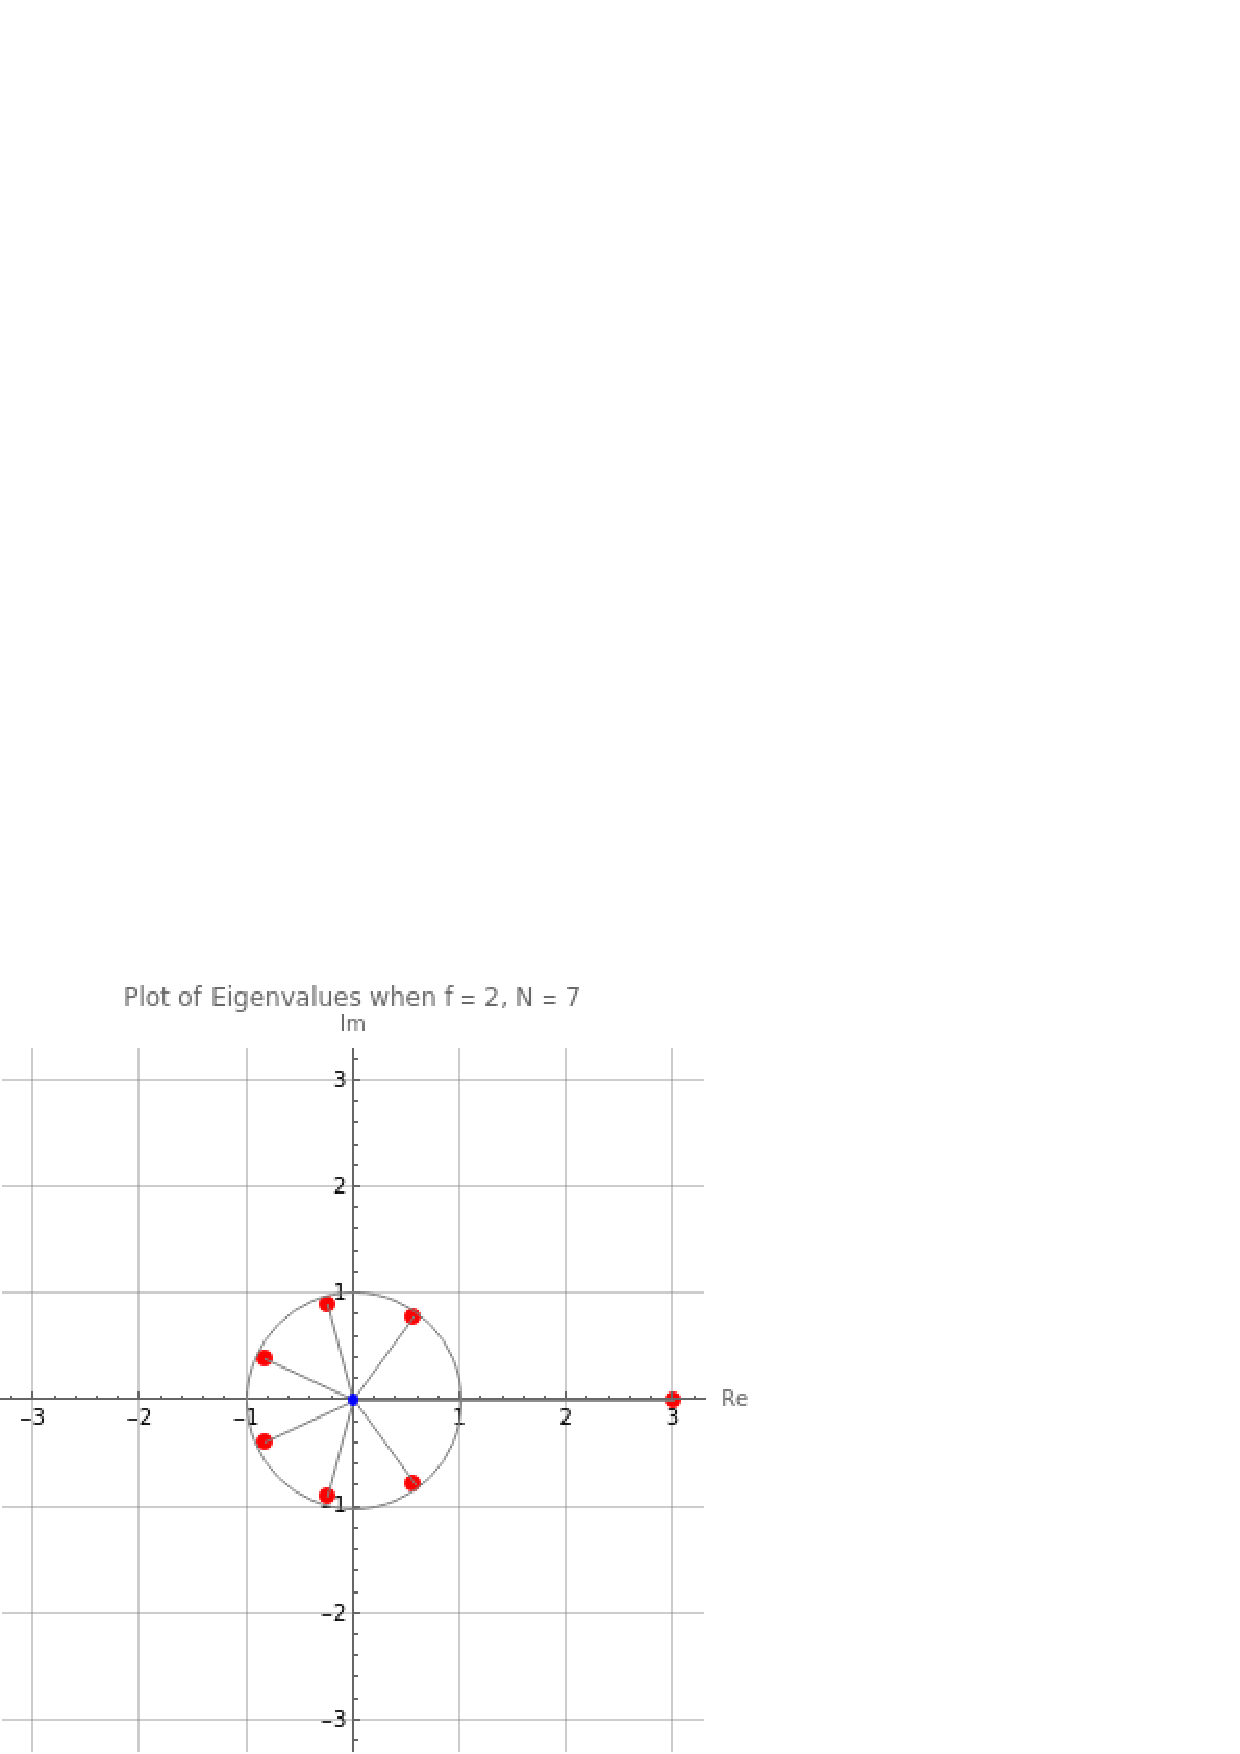
\includegraphics[width=\textwidth]{f2N7.png}
        \caption{$f > 1$, $N$ odd}
        \label{fig:fig1}
    \end{subfigure}
    \hfill
    \begin{subfigure}[b]{0.45\textwidth}
        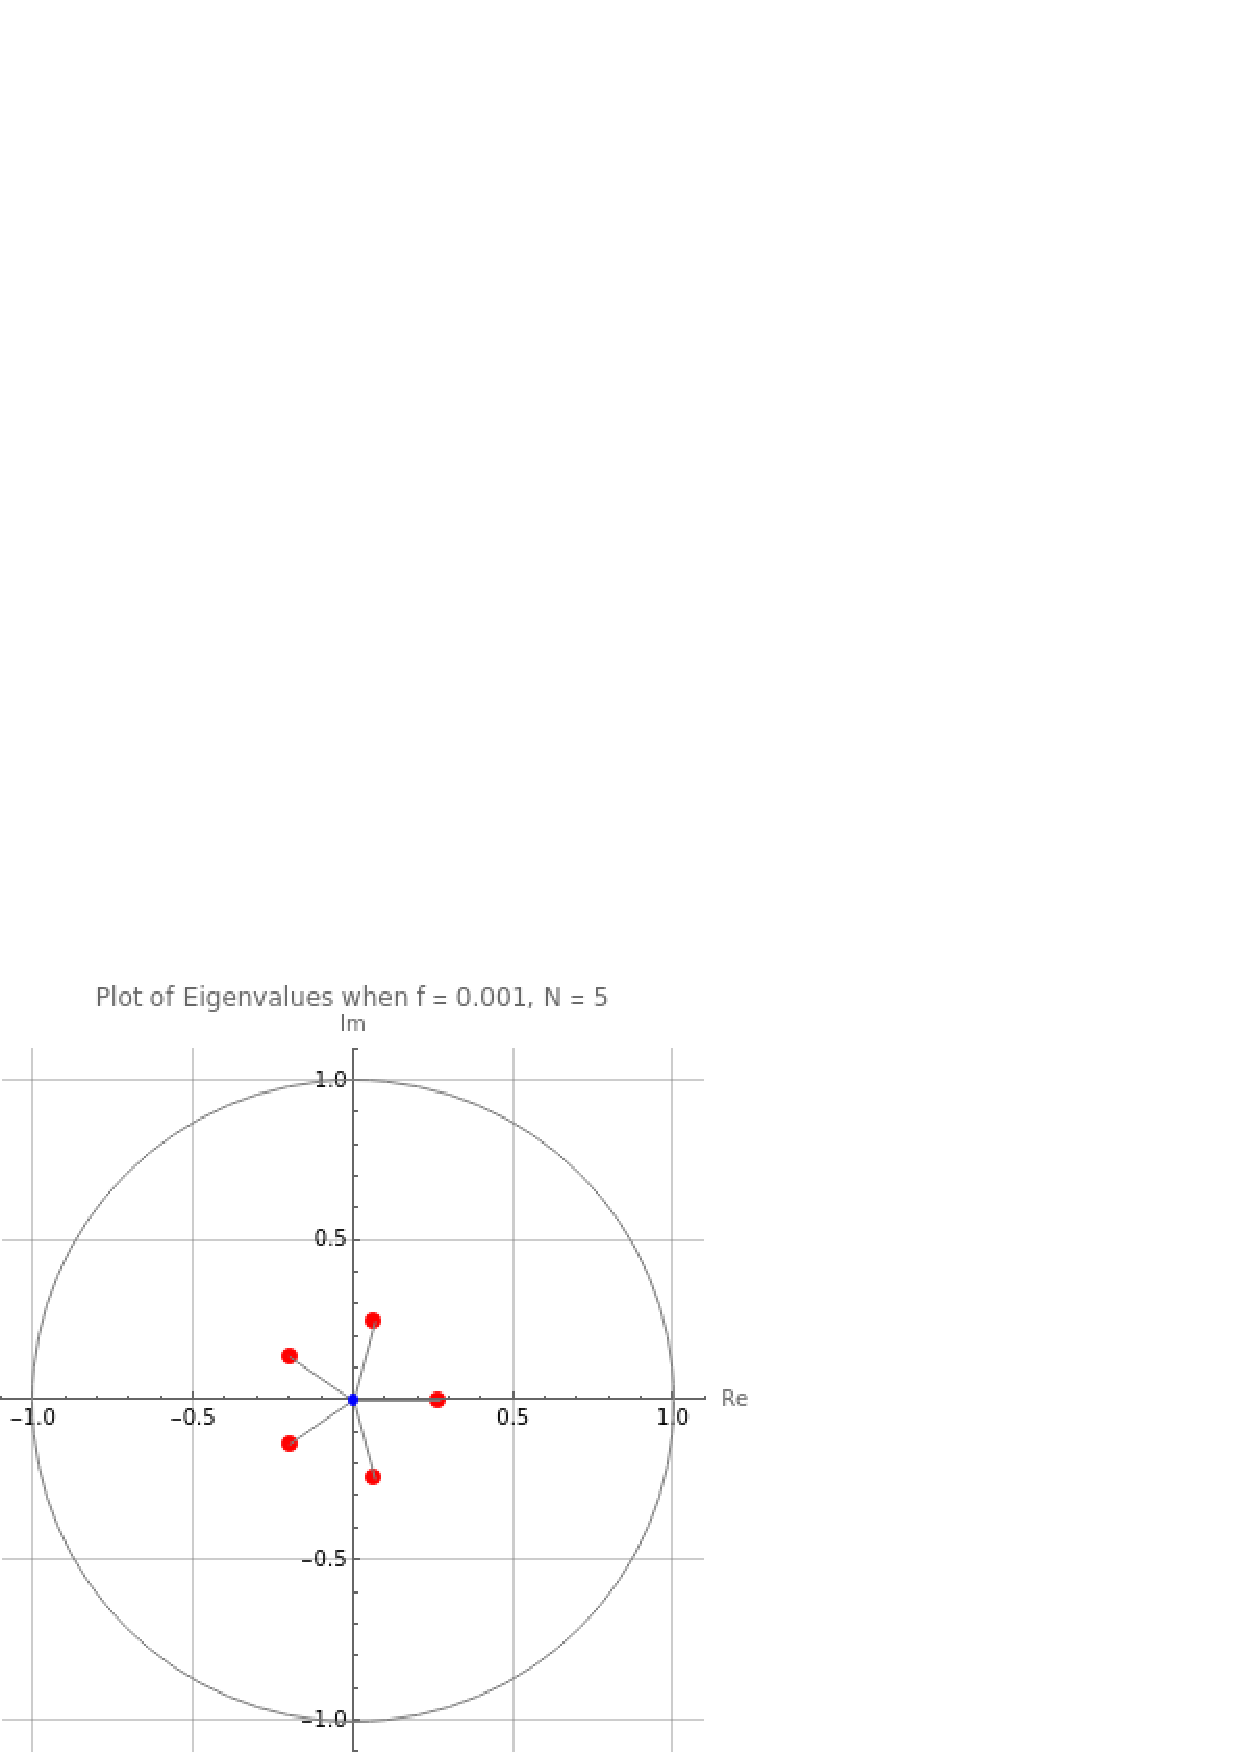
\includegraphics[width=\textwidth]{fsmN5.png}
        \caption{Small fertility rate}
        \label{fig:fig2}
    \end{subfigure}
    \\
    \begin{subfigure}[b]{0.45\textwidth}
        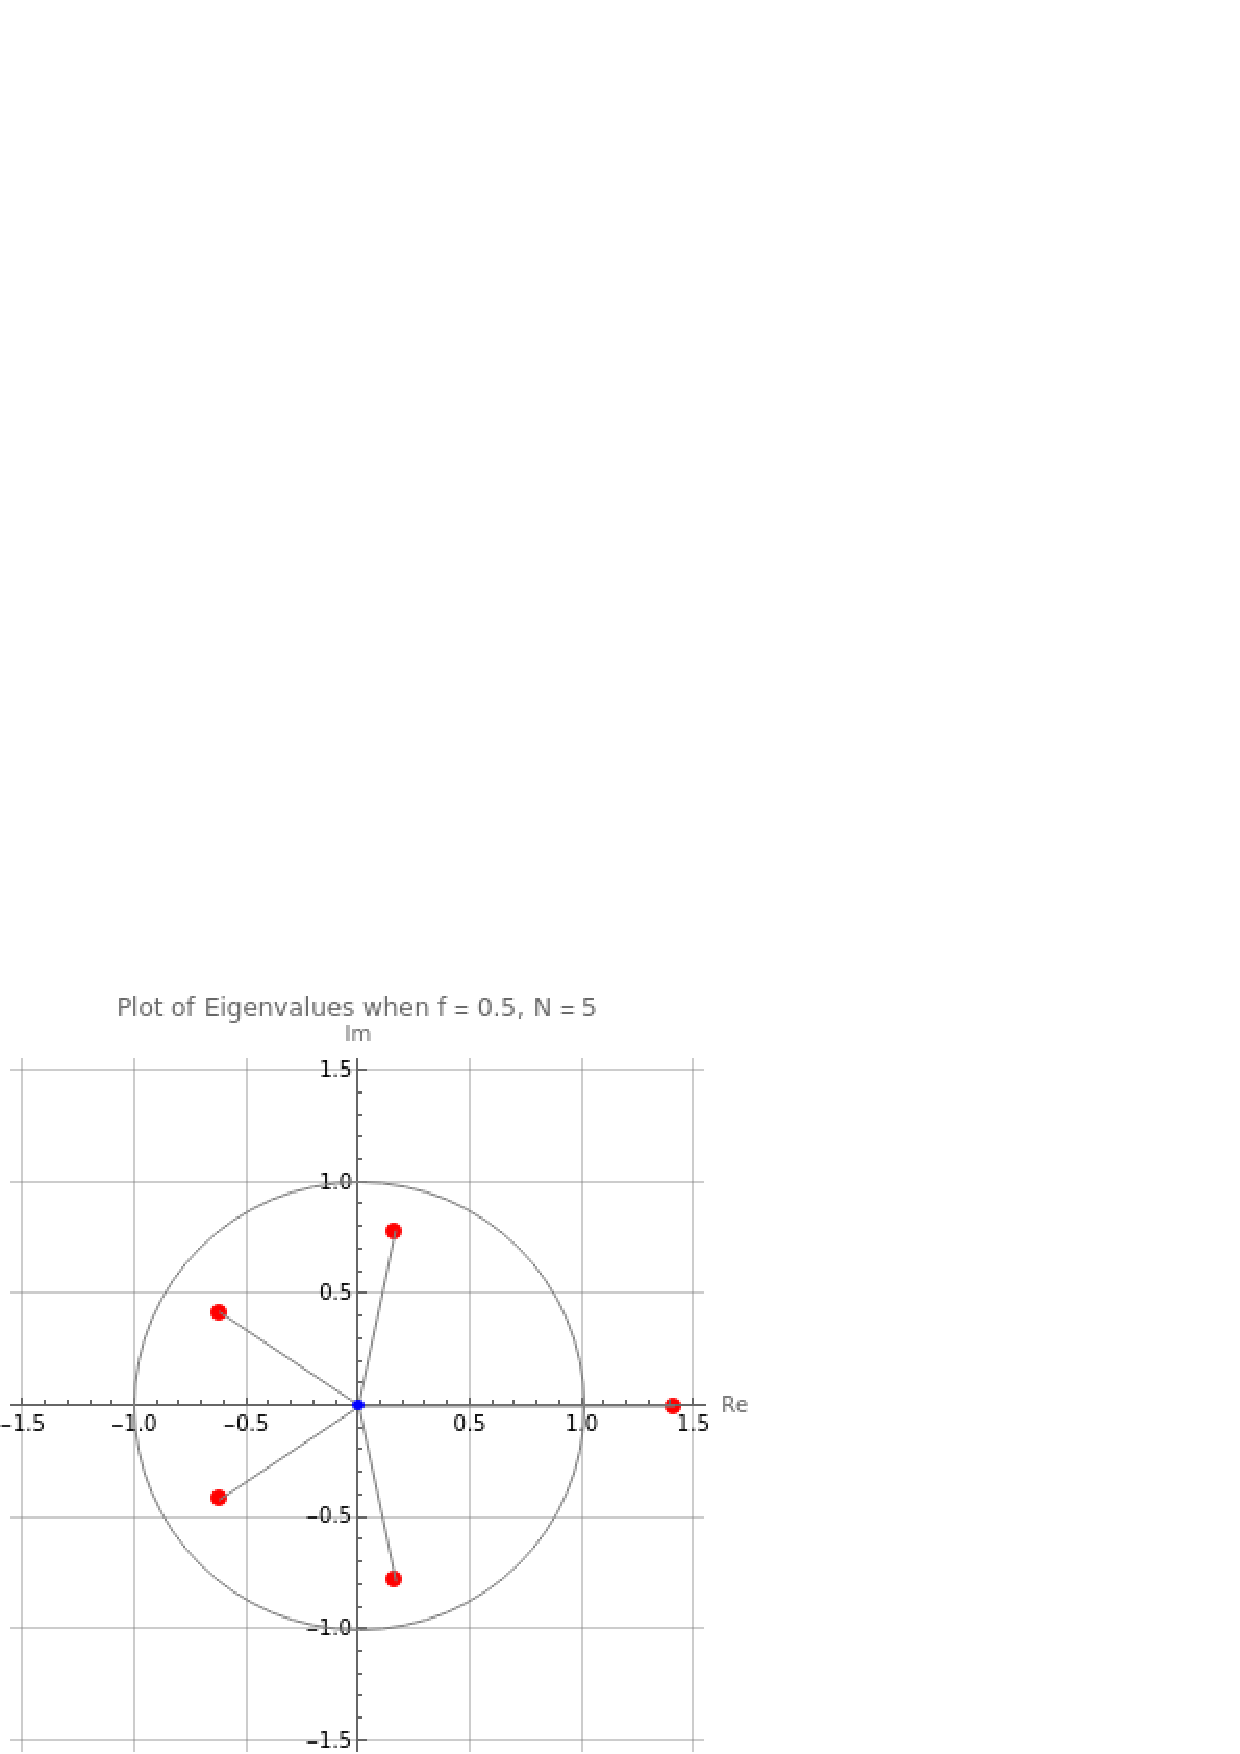
\includegraphics[width=\textwidth]{fHfN5.png}
        \caption{$f < 1$}
        \label{fig:fig3}
    \end{subfigure}
    \hfill
    \begin{subfigure}[b]{0.45\textwidth}
        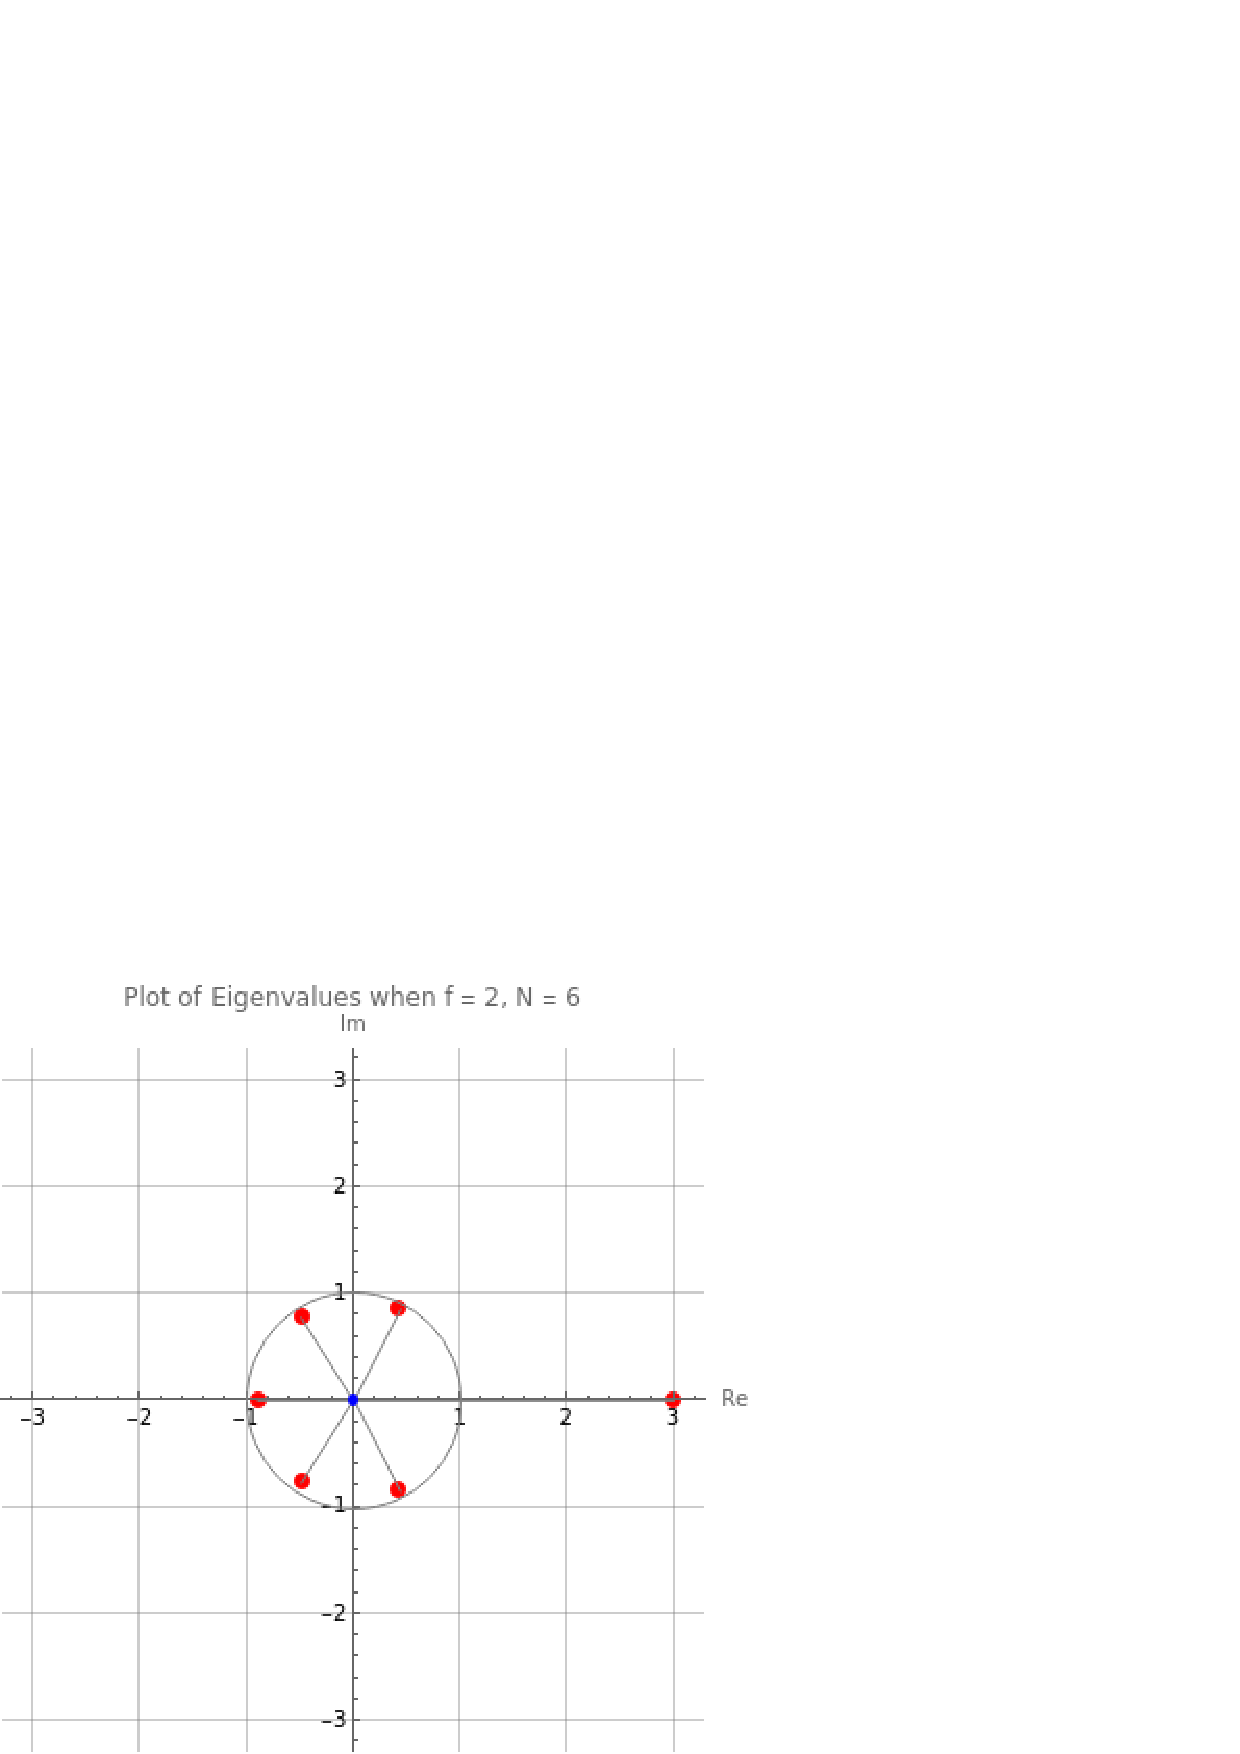
\includegraphics[width=\textwidth]{f2N6.png}
        \caption{$f > 1$, $N$ even}
        \label{fig:fig4}
    \end{subfigure}
    \caption{Complex Eigenvalues of Simple Leslie Matrices for varying $f, N$.}
    \label{fig:overall}
\end{figure}

\newpage

\begin{cor}[Real Root of the Characteristic Equation]

    The real root of the characteristic equation has a magnitude greater 
    than $1$ if and only if $1-fN < 0$. 
\end{cor}
\begin{proof}
    We know that $\ch_(z)$ can be evaluated somewhere in 
    the interval $[1, \infty)$ to be positive. 
    Evaluate the following:
    \begin{equation}
        \ch_N(1) \ =\  1 - fN. 
    \end{equation}
    If this value is less than zero, than the real 
    root lies somewhere in the range $(1, \infty)$. 
    Otherwise, since $f(0) < 0$, the dominant root 
    must be less than $1$. 
\end{proof}



With a little more analysis, we provide a lower bound and the 
upper bound of the maximum eigenvalues of $L_f$. 

\begin{theorem}[Bounds for the maximum eigenvalue]\label{thm:Bound}

 Given that $1-fN \leq 0$, the maximum eigenvalue of $L_f$ of order 
 $N$ is given by 
 \[
 1 + f - \frac 1 {N} \ \leq\ \lambda_{\rm max} \ < \ 1 + f.
 \]
\end{theorem}

\begin{proof}
    The upper bound is trivial:
    \[
        \ch_N(1+f) \ = \ f \ >\  0.
    \]  
    We have $\ch_N(0) = -f < 0$, and thus by the Intermediate Value Theorem the maximum root is 
    bounded. 

    To obtain the lower bound, we write $f = 1/N + \epsilon$ for 
    some $\epsilon \geq 0$. With some algebra, we compute $\ch_N(z)$ at the lower 
    bound. If we show that this value is less than zero, the 
    dominating root must be greater than the purported lower bound. We find
    \[
        \ch_N\left(
            1 + f - \frac 1 N
        \right)  \ = \ -
        \left(
            1 + f - \frac 1 N
        \right)^N \left[
            \frac {1} {fN - 1}
        \right]
        + \frac {fN} {fN - 1}.
    \]
    We wish to bound this value by zero. It suffices to show 
    \[
        fN - \left(
            1 + f - \frac 1 N
        \right)^N \ \leq\ 0,
    \]
    Which, using the $\epsilon$ substitution converts to 
    \[
        1 + N\epsilon - (1 + \epsilon)^N \ \geq \ 0.
    \]
    Expanding the power term by the binomial theorem, 
    we see the inequality holds. 
\end{proof}

% %%%%%%%%%%%%%%%%%%%%%%%%%%%%%%%%%%%%%%%%%%%%%%%%%%%%%%%%%%%%%%%%%%%%%%%%%%%%%%%%%%%%%%%%%%%%%%%%%%%%%%%%%%%%%%%%%%%%%%%%%%%%%%%%%%%%
% 

\section{The Leslie Predator-Prey Model}

\subsection{The Classic 
Lotka-Volterra Model}
Let $x(t), y(t)$ be continuous functions 
that describe the density of the prey and predator. That is, the range of $x, y$ are in the interval $[0, 1]$. The classical Predator-Prey Model is described by a system of differential equations. 
\begin{eqnarray}
    \frac{dx}{dt} &=& 
    rx(1-x) - axy \nonumber\\ 
    \frac {dy}{dt} &=& 
    ay(x-y)
\end{eqnarray}
The focus of study for the classical model is to find out the conditions 
for when the system reaches stability. In \cite{Mer10}, Merdan studies a 
similar system that accounts for the Allee effect, described by the equations below. 
\begin{eqnarray}
    \frac {dx}{dt} & = & r\alpha(x) x (1-x) - axy \nonumber \\ 
    \frac {dy}{dt} & = & ay(x - y)
\end{eqnarray}
The term $\alpha(x) := x/(\beta + x)$ is the term for the Allee effect. Merdan shows that under the condition 
\begin{eqnarray}
    r - \alpha \beta  \ > \ 0 
\end{eqnarray}
the population converges to a 
positive stable state 
\begin{eqnarray}
    (x_*, y_*) \ := \ ((r - \alpha\beta)/(a + r), (r-\alpha\beta)/(a + r)) 
\end{eqnarray}

\subsection{The Predator-Prey Model with Leslie Matrices}\label{sec:PPmodels}

We wish to account for the different age groups in the predator and prey population. Hence, we replace the population density, which was a scalar function, into a vector. Also, we replace the reproductive and predation constants by a Leslie matrix. 

\begin{definition}[Leslie Predator-Prey]
Let $\vec \alpha_n$, $\vec \beta_n \in \mathbb R_{\rm pos}^N$ be the population vectors 
of the predator and prey at timestep $n$. 
Set the number of age groups of both population to be 
$N$, so the population vectors will have entries. 
\begin{eqnarray}
    \vec \alpha_n \ = \ (\alpha_n^{(1)}, \dots, \alpha_n^{(N)}) 
    \nonumber \\
    \vec \beta_n \ = \ (\beta_n^{(1)}, \dots, \beta_n^{(N)}) .
\end{eqnarray}
 The population 
vectors are defined by the following 
system of matrix differences:
\begin{eqnarray}
    \vec \alpha_{n + 1} &=& L_a \vec \alpha_n + k m \vec \beta_n \nonumber \\ 
    \vec \beta_{n + 1} &=& L_b \vec \beta_n - k \vec \alpha_n.
\end{eqnarray}
The constants $k, m$ are predation ratio and nurturing ratios, both greater than zero. 
We set the population of predator and prey to be the sum 
of all entries. In symbols, we write $P_{a, n}, P_{b, n}$ the population 
of the predator and prey by the following sums. 
\begin{equation}
    P_{a, n} \ = \ \sum_{k = 1}^{N} \alpha^{(k)}_{n}  
    ,
    P_{b, n} \ = \ \sum_{k = 1}^{N} \beta^{(k)}_{n} 
\end{equation}
\end{definition}


We assume that the $x$-value of $L_\alpha$ is less than $1/2$ 
and that the $x$-value of $L_\beta$ is greater than $1/2$. In 
other words, the predator population decays in absense of the prey 
and the prey populatin explodes in absence of the predator. 
Moreover, the population is fixed to be nonnegative. 

If the population reaches zero 
at some time $n \in \mathbb{Z}_{\rm pos}$, 
we say that the population has gone 
extinct. 
Notice that if the predation rate is too high, the prey population 
will be exhausted. In the absence of the prey, the predator 
population will become extinct. On the other hand, if the predation 
rate is too low, the predator population will not be able to maintain 
itself, and will become extinct. Hence, it is natural to ask 
the following question. 

\begin{problem}[Optimal Predation Strategy]
What ranges of the real value $k$ guarantees exponential growth 
of the predator? Moreover, what value of $k$ is necessary to guarantee 
maximum growth?
\end{problem}

Furthermore the real-valued formula motivates us to study the complex-valued model. 

\begin{definition}[Complex Predator-Prey]\label{thm:complexModel}
Let 
 $\alpha_n, \beta_n \in \mathbb R_{\rm pos}^N$ for $n = 0$
$\alpha_n, \beta_n \in \mathbb C^N$ for $n > 0$ be the population vectors 
of the predator and prey at timestep $n$. The population 
vectors are defined by the following 
system of matrix differences. 
\begin{eqnarray}
    \vec \alpha_n \ = \ (\alpha_n^{(1)}, \dots, \alpha_n^{(N)}) 
    \nonumber \\
    \vec \beta_n \ = \ (\beta_n^{(1)}, \dots, \beta_n^{(N)}).
\end{eqnarray}
 The population 
vectors are defined by the following 
system of matrix differences: 
\begin{eqnarray}
    \vec \alpha_{n + 1} &=& iL_a \vec \alpha_n + k m \vec \beta_n \nonumber \\ 
    \vec \beta_{n + 1} &=& iL_b \vec \beta_n - k \vec \alpha_n,
\end{eqnarray}
where $k, m$ are predation ratio and nurturing ratios, both greater than zero, for we set the population of predator and prey to be the sum 
of all entries. In symbols, we write $P_{a, n}, P_{b, n}$ the population 
of the predator and prey by the following sums:
\begin{equation}
    P_{a, n} \ = \ \left\|\sum_{k = 1}^{N} \alpha^{(k)}_{n} \right\|
    ,
    P_{b, n} \ = \ \left\|\sum_{k = 1}^{N} \beta^{(k)}_{n} \right\|
\end{equation}
\end{definition}

Experimentally speaking, for the complex model, the population 
grows almost surely unless the predation rate $k$ is zero. The natural 
question to ask for this model is the following. 

\begin{problem}[Modeling Predator Growth]
    What is the growth rate of the predators as $n \rightarrow \infty$?
\end{problem}

%Might add the winner-takes all thm?

By elementary substitutions, we obtain the following proposition. 

\begin{prop}[Coupled 1st order to 2nd order]\label{thm:to2ndOrd}
Assuming both 
the prey and predator population are nonextinct within 
a given period of time, 
the predator population satisfies the following second order 
difference equation:
\begin{eqnarray}
\alpha_n \ =\ (L_a + L_b) \alpha_{n - 1} - L_b L_a \alpha_{n -2} - m k^2 \alpha_{n - 2} \nonumber
\\
\beta_n \ =\ (L_b + L_a) \beta_{n - 1} - L_a L_b \beta_{n -2} - m k^2 \beta_{n - 2}.
\end{eqnarray}
For the complex model, 
\begin{eqnarray}
\alpha_n = i(L_a + L_b) \alpha_{n - 1} + L_b L_a \alpha_{n -2} - m k^2 \alpha_{n - 2} \nonumber
\\
\beta_n = i(L_b + L_a) \beta_{n - 1} + L_a L_b \beta_{n -2} - m k^2 \beta_{n - 2}. \label{cmplx_model}
\end{eqnarray}
\end{prop}


The coupled second order difference equation can be solved using 
generating function under the assumption that the Leslie Matrices 
of the two populations are constant multiples of each other. 

\begin{theorem} [Generating Function of the predator population for the real case]
    Suppose $\vec \alpha_n$ is the population vector 
    of the predator in a real Leslie Predator-Prey model where 
    $L = \rho L$ and $L_b = L$. 
    The generating function of $\vec \alpha_n$ is
    \begin{equation}
        G(x) \ = \ 
\frac{ \left(\rho L + m k^2 - (\rho + 1) L x\right)\vec \alpha_0 + (\rho L + m k^2) x \vec  \alpha_1}{x^2 - x(\rho + 1) L + \rho L^2 + m k^2}.
    \end{equation}
\end{theorem}

\begin{proof}
    From the recurrence relation provided in Proposition \ref{thm:to2ndOrd}, 
    we have the following identity: 
    \begin{equation}
        \begin{split}
        \left[x^2 - x (\rho + 1) L + (\rho L^2 + mk^2)\right]G(x) \\ = \  
        -(\rho + 1) L \vec \alpha_0 x 
        +(\rho L^2 + mk^2) \vec \alpha_0 
        + (\rho L^2  + m k^2) \vec \alpha_1 x
        \end{split}.
    \end{equation}
    This identity can be verified by substituting $G(x)$ and 
    imposing the conditions on $\alpha_n$. The expansion on the 
    lefthand side has residues for terms that have an $x$ power 
    less than or equal to 2. Solve for $G(x)$ to obtain the result. 
\end{proof}


Using partial fraction decomposition, it is possible to obtain 
a closed form expansion for $\vec \alpha_n$. 

\begin{theorem} [Formula for $\vec \alpha_n$]
    For $\vec \alpha_n$ where $n > 0$, 
    \begin{equation}
    \vec \alpha_n \ = \ 
    \frac {
(L^2 \rho + k^2 m)^{n - 2}
    } {\sqrt D} 
    \left[
        \left(
            (k^2m + L^2 \rho) \vec \alpha_1 - L(1 + \rho) 
\left(
            k^2m + L^2\rho
        \right)
            \vec \alpha_0
        \right)\delta_{n - 1}
        + \left(
            k^2m + L^2\rho
        \right)^2\vec \alpha_0 \delta_{n}
    \right]
    \end{equation}
    where $D$ is defined by
    \begin{equation}
        D \ = \ L ^2 (1 + \rho)^2 - 4 (mk^2 + \rho L^2)
    \end{equation}
    and the sequence $\delta_n$ is defined by 
    \begin{equation}
        \delta_n \ = \ 
        \left(
            \frac 1 2
        \right)^n 
        \left(
                L^2 \rho + k^2 m
        \right)^{-n}
        \left[
            \sum_{\substack{l = 1 \\ l \textnormal{ odd}}}^{n + 1}
            \binom{n + 1}{l} 
            [L(1+\rho)]^{t + 1 - l}(\sqrt D)^l
        \right]
    \end{equation}
\end{theorem}

\begin{proof}
    The derivation follows by applying partial fraction decomposition on the 
    Generating Function. 
\end{proof}

Though the theorem gives a closed-form equation for the population, 
the complexity of the formula poses difficulties to determine the optimal 
predation rate for maximal growth.

\subsection{Real-Valued Model with Scalar $L$}\label{sec:scalarModel}
%solution for scalars


The following three propositions properly model 
the populations where the dimension of the Leslie matrix 
is 1. That is, the population growth is characterized 
by an exponential of a scalar without interaction. 
To emphasize the scalarness, we write $l_a < 1$ and $l_b > 1$ 
instead of $L_a, L_b$. 

\begin{theorem}[Eigenvalues of the companion matrix]\label{thm:simpleEval}
Using Proposition \ref{thm:to2ndOrd}, we write the companion matrix that 
describes the populations. 
\[
    \twobytwoMat(
        l_a + l_b, -l_a l_b -k^2 m, 1, 0
    ).
\]
The eigenvalues of this matrix is purely real if and only if 
\begin{equation}
    k \ \leq\  \frac {l_a - l_b} {2\sqrt{m}}.
\end{equation}
Otherwise, the eigenvalues of these matrices are complex conjugates 
of each other. 
\end{theorem}

\begin{proof}
    The characteristic equation of the companion matrix is 
    \[
        \lambda ^2 - (l_a + l_b) \lambda + k^2m + l_a l_b.
    \]
    For the eigenvalues to be purely real, the discriminant $D$ of this polynomial must be a nonnegative value:
    \begin{equation}
        \frac D 4 \ :=\ \frac {(l_a + l_b)^2} 4 - k^2m + l_a l_b \ \geq \ 0
    \end{equation}
    With elementary algebra, we obtain 
    \begin{equation}
    k \ \leq\ \frac {l_a - l_b} {2\sqrt{m}}. 
    \end{equation}
    Otherwise, if $D/4 < 0$ then the eigenvalue will have an imaginary part, and the two eigenvalues will be complex conjugates of each other. 
\end{proof}



\begin{theorem}[Exponential growth of population for small predation]
The following condition guarantees that the predator and prey population 
do not vanish as $n \rightarrow \infty$: 
\begin{equation}
    k \ \leq \ \sqrt{
        \frac {(1 - l_b)(l_a - 1)} {m}
    }.
\end{equation}
\end{theorem}

\begin{proof}
    Assume that the discriminant is a nonnegative real value. Then 
    the maximum eigenvalue must be 
    \begin{equation}
        \frac {l_a + l_b} 2 + \frac {\sqrt D} 2,
    \end{equation}
    which must be greater or equal to 1 for the population to not vanish. 
\end{proof}

\begin{theorem}[Complex eigenvalue implies extinction]
If 
\begin{equation}\label{eqn:simpleVanish}
    k \ > \  \frac {l_a - l_b} {2\sqrt{m}}
\end{equation}
then the population is guaranteed to go extinct. 
\end{theorem}
\begin{proof}
    It follows trivially that the condition (\ref{eqn:simpleVanish}) 
    implies that the eigenvalue is complex. Also, the real part of the root will be $(l_a + l_b)/2$ which is guaranteed to be positive. Let the two eigenvalues of the companion matrix be $\gamma$ and $\gamma *$ with 
    \begin{equation}
    \gamma \ = \ r e^{i \theta} ,\ \gamma* \ = \ r e^{-i \theta} 
    \end{equation}
    where $r > 0$,
    $\theta \in (0, \pi/2)$. By Proposition \ref{thm:to2ndOrd}, we note that the population of 
    the predator at time $n$ can be written as 
    \begin{equation}\label{eqn:gammaPopulation}
    \alpha_n \ = \ \nu_1 \gamma^n + \nu_2 (\gamma*)^n.
    \end{equation}
    We also observe that the population $\alpha_0, \alpha_1$ can be assumed to be a positive real value. If $\alpha_1 \leq 0$, then the population has gone extinct at time 1. 
    Equation \ref{eqn:gammaPopulation} for $n = 0, 1$ is 
    \begin{eqnarray}
    \alpha_0 & = & \nu_1 + \nu_2 \nonumber\\ 
    a_1 & = & \nu_1\gamma + \nu_2\gamma*
    \end{eqnarray}
    Since $\alpha_0, \alpha_1 > 0$, we deduce that $\nu_1 = \nu_2 := \nu/2 > 0$. Finally, we rewrite the population at time $n$. 
    \begin{equation}
    \alpha_n \ = \ \Re (\nu \gamma ^n) = \nu r^n \cos(n\theta)
    \end{equation}
    We know that $\theta \in (0, \pi / 2)$. Thus, there exists 
    an integer $n$ such that $\cos(n\theta) < 0$. We have shown that the predator population must go extinct. 
\end{proof}
\hfill \qed

\subsection{The Complex-Valued Model with $L_a = \rho L_b$}
%Special solution for leslie Matrices

To solve the second order matrix 
recurrence related to 
the predator-prey model, 
we solve a characteristic equation 
where the coefficients are Matrices. 
Since the only Matrices involved on this equation are $I$ and $L_\beta$
which commute, we can use the quadratic equation to solve this equation. 


\begin{theorem}[Maximum Eigenvalue for the general case]\label{eqn:MaxEvalGen}
    The population vector of the predator in (\ref{LeslieDef}) 
    can be characterized as 
    \begin{equation}
    \vec \alpha_n \ =\ \Lambda_1^{n}  \vec v_1+ \Lambda_2^{n}\vec v_2
    \end{equation}
    for some vectors $\vec v_1$ and $\vec v_2$. The 
    growth of the predator population 
    is dominated by the maximum eigenvalue 
    of $\Lambda_1$. Call the maximum eigenvalue of $L_b$ 
    as $\lambda_{\rm max}$. Then, the maximum eigenvalue of $\Lambda_1$, 
    denoted by $\Lambda_{\rm max}$ has the following modulus. 
    \begin{equation}
        \|\Lambda_{\rm max} \| \ =\   \frac {
            (\rho + 1)\lambda_{\rm max} + \sqrt{(\rho + 1)^2 \lambda_{\rm max}^2 + 4mk^2}
        } 2
    \end{equation}. 
\end{theorem}
\begin{proof}
    It is possible to solve for $\Lambda_1, \Lambda_2$ directly. 
We wish to find a matrix $\Lambda$ such that 
\begin{equation}
\Lambda^2 - i(\rho + 1) L_b \Lambda + \rho L_b^2+ mk^2 I = 0
\end{equation}
    Apply the quadratic formula. 
    \begin{eqnarray}
        \Lambda_1 \ = \ 
        \frac {
        (1 + \rho) L_b^2 + 
        \sqrt{
        (1-\rho)^2L_b^2 + 4mk^2
        }
        } 2 i \nonumber \\ 
 \Lambda_2 \ = \ 
        \frac {
        (1 + \rho) L_b^2 - 
        \sqrt{
        (1-\rho)^2L_b^2 + 4mk^2
        }
        } 2 i. 
    \end{eqnarray}
    The magnitude of $\Lambda_1$ is greater than that of $\Lambda_2$. 
    We approximate the population of the predator at the limit $n \rightarrow \infty$. 
    \begin{eqnarray}
        P_{a, n} \ = \ \|\vec a_n\| \ = \ 
        \|\Lambda_1\|^n \|\vec v_1\| + 
 \|\Lambda_2\|^n \|\vec v_2\| 
 \ \approx  \ 
\|\Lambda_1\|^n \|\vec v_1\|
    \end{eqnarray}
    It remains to show that the vector $\vec v_1$ is nonzero. Assume for a contradiction that $\vec v_1 = (0, \dots, 0)$. Then we can write out the predator population at time 0, 1 as 
    \begin{equation}
    \vec \alpha_0 \ = \ \vec v_2, \ \vec \alpha_1 \ = \ \Lambda_2 \vec v_2 
    \end{equation}
    which indicates that 
    \begin{equation}
    \vec \alpha_1 \ = \ \Lambda_2 \vec \alpha_0
    \end{equation}
    and since $\Lambda_2$ is purely imaginary, $\alpha_1$ is also purely imaginary. 
    The initial condition of the model in Definition \ref{thm:complexModel} 
    dictates that each entry of $\vec \alpha_0, \vec \beta$ is a positive real and that 
    \begin{equation}
    \vec \alpha_1 \ = \ iL_{\alpha} \vec \alpha_n + km \vec\beta_n.
    \end{equation}
    Therefore $\alpha_1 $ cannot be purely imaginary, which is a contradiction. 
\end{proof}


%%%%%%%%%%%%%%%%%%%%%%%%%%%%%%%%%%%%%%%%%%%%%%%%%%%%%%%%
%%%%%%%%%%%%%%%%%%%%%%%%%%%%%%%%%%%%%%%%%%%%%%%%%%%%%%%%
%%%%%%%%%%%%%%%%%%%%%%%%%%%%%%%%%%%%%%%%%%%%%%%%%%%%%%%%
%%%%%%%%%%%%%%%%%%%%%%%%%%%%%%%%%%%%%%%%%%%%%%%%%%%%%%%%
%%%%%%%%%%%%%%%%%%%%%%%%%%%%%%%%%%%%%%%%%%%%%%%%%%%%%%%%
%%%%%%%%%%%%%%%%%%%%%%%%%%%%%%%%%%%%%%%%%%%%%%%%%%%%%%%%
%%%%%%%%%%%%%%%%%%%%%%%%%%%%%%%%%%%%%%%%%%%%%%%%%%%%%%%%
%%%%%%%%%%%%%%%%%%%%%%%%%%%%%%%%%%%%%%%%%%%%%%%%%%%%%%%%
\section{The Competitive Model}
We can slightly modify one of the sign of the model and 
study the following system. Suppose there exists two identical 
population that has a same growth matrix $L$. Also, assume 
that the population is nonvanishing without interaction. That is, 
$\lambda_{max}$, the maximum eigenvalue of $L$ is greater 
than or equal to 1. 
\begin{definition}[Leslie Competitive Model]
Let $\alpha_n$, $\beta_n$ be the population vectors 
of the predator and prey at timestep $n$. The competitive 
model is defined by the following 
system of matrix differences. 
\begin{eqnarray}\label{eqn:conditions}
    \alpha_{n + 1} &=& \max(L \alpha_n - k m \beta_n, \vec 0) \\ 
    \beta_{n + 1} &=& \max(L \beta_n - k \alpha_n, \vec 0) \nonumber
\end{eqnarray}
$k, m$ are interaction ratio and competitive advantage, both between $0, 1$. 
\end{definition}



\subsection{Last Species Standing}\label{sec:lastSpecies}

A similar analysis used for the predator-prey model 
can be applied to yield the following result. 

\begin{theorem}[Last Species Standing]
    Suppose $\vec \alpha_0 = \alpha_0 (1, \dots, 1)$ and 
    $\vec \beta_0 = \beta_0 (1, \dots, 1)$.
    In a Leslie competetive model, one of the two 
    species is likely to vanish as $n \rightarrow \infty$  
    The fate of the species is determined 
    by the sign of the term 
    \begin{equation}
        D \ :=\ \alpha_0 - \sqrt{m} \beta_0.
    \end{equation}
    . In particular, if $D > 0$ then the population $\alpha$ 
    vanishes and population $\beta$ grows exponentially.
     If $D < 0$, then the population $\beta$ vanishes and the population $\alpha$ 
     grows exponentially. 
    If $D = 0$, either both species vanish or grow exponentially together. 
\end{theorem}
\begin{proof}
    Proposition \ref{thm:to2ndOrd} can be simply generalized by 
    the substitution \newline $m \mapsto -m$. From the recursive relation 
    \begin{equation}
        \alpha_n \ = \ (2L)\alpha_{n - 1} -L^2 \alpha_{n - 2} + mk^2 \alpha_{n - 2}
    \end{equation}
    we obtain the characteristic eqation 
    \begin{equation}
    \Lambda ^2 - 2L \Lambda + L^2 - mk^2 \ =\ 0
    \end{equation}
    and by the quadratic formula, we derive the root. 
    \begin{eqnarray}
        \Lambda_1 \ = \ L + k\sqrt{m} I 
        \nonumber \\
        \Lambda_2\ = \ L - k\sqrt{m} I
    \end{eqnarray}
    where $I$ is the identity matrix. 
    Notice that $k, m$ are both nonnegative real values, and $L$ 
    is assumed to guarantee positive population growth. Hence, 
    $\Lambda_1$ has a positive eigenvalue. 

    From (\ref{eqn:MaxEvalGen}), we characterize the population as
    \begin{equation}\label{eqn:closedEq}
    \vec \alpha_n \ =\ \Lambda_1^{n}  \vec v_1+ \Lambda_2^{n}\vec v_2
    \end{equation}
    In the limit as $n \rightarrow \infty$, 
    \begin{equation}
    \vec \alpha_n \ \approx\ \Lambda_1^{n}  \vec v_1
    \end{equation}
    Thus, the population is nonvanishing if and only if $\vec v_1$ 
    is positive. We compute $\vec v_1$ directly. From \ref{eqn:closedEq}, we obtain two conditions: 
    \begin{eqnarray}
        \vec \alpha_0 & = & \vec v_1 + \vec v_2 \nonumber \\ 
        \vec \alpha_1 & = & \Lambda_1 \vec v_1 + \Lambda_2 \vec v_2.
    \end{eqnarray}
    Solving for $\vec v_1$, obtain 
    \begin{equation}
        \begin{split}
        \vec v_1 \ = \ \frac {\Lambda_2 \vec\alpha_0 - \vec\alpha_1} {\Lambda_2 - \Lambda_1}
        \ = \ 
        \frac {L\vec \alpha_0 - k\sqrt m \vec \alpha_0 - L \vec \alpha_0 + km\beta_0} {2mk} 
        \ = \ 
        \frac {\sqrt{m}\vec\beta_0 -  \vec \alpha_0} {2\sqrt m} \\ 
        \ = \ \frac {\sqrt m \beta_0 - \alpha_0} {2 \sqrt m} (1, \dots, 1) 
        \ = \ -\frac D{2\sqrt m} (1, \dots, 1).
        \end{split}
    \end{equation}
    Similarly, we obtain 
    \begin{equation}
        \beta_n \ \approx \ \Lambda_1 \vec w_1  
    \end{equation}
    where 
    \begin{equation}
        \ = \ \frac D {2\sqrt m }(1, \dots, 1).
    \end{equation}
    . If $D \neq 0$, plugging in the appropriate value of $D$ yields 
    the result. Suppose $D = 0$ or $\alpha_0 = \sqrt m \beta _0$. The 
    conditions of \ref{eqn:conditions} imply
    \begin{eqnarray}
        \vec \alpha_1  \ = \ L \vec \alpha_0 - k \sqrt m \vec \alpha_0 \nonumber \\ 
        \vec \beta_1 \ = \ L \vec \beta_0 - k \sqrt m \vec \beta_0.
    \end{eqnarray} 
    By induction, it is possible to prove that 
    \begin{eqnarray}
        \vec \alpha_n \ = \ \sqrt m \vec \beta_n
    \end{eqnarray}
    for all nonnegative integers $n$. In turn, we obtain 
    \begin{eqnarray}
        \vec \alpha_{n + 1} \ = \ 
        \left(
            L - k \sqrt m
        \right)^n \vec \alpha_0 \nonumber
        \\ 
        \vec \beta_{n + 1} \ = \ 
        \left(
            L - k \sqrt m
        \right)^n \vec \beta_0,
    \end{eqnarray}
    and the population grows or vanishes simultaneously. 
\end{proof}


\section{The Migration Model}
\section{Potential Use of Quantum Operators}
\section{Future Work}


 \appendix
% %%%%%%%%%%%%%%%%%%%%%%%%%%%%%%%%%%%%%%%%%%%%%%%%%%%%%%%%%%%%%%%%%%%%%%%%%%%%%%%%%%%%%%%%%%%%%%%%%%%%%%%%%%%%%%%%%%%%%%%%%%%%%%%%%%%%
% %%%%%%%%%%%%%%%%%%%%%%%%%%%%%%%%%%%%%%%%%%%%%%%%%%%%%%%%%%%%%%%%%%%%%%%%%%%%%%%%%%%%%%%%%%%%%%%%%%%%%%%%%%%%%%%%%%%%%%%%%%%%%%%%%%%%
% %%%%%%%%%%%%%%%%%%%%%%%%%%%%%%%%%%%%%%%%%%%%%%%%%%%%%%%%%%%%%%%%%%%%%%%%%%%%%%%%%%%%%%%%%%%%%%%%%%%%%%%%%%%%%%%%%%%%%%%%%%%%%%%%%%%%






%%%%%%%%%%%%%%%%%%%%%%%%%%%%%%%%%%%%%%%%%%%%%%%%%%%%%%%%%%%%%%%%%%%%%%%%%%%%%%%%%%%%%%%%%%%%%%%%%%%%%%%%%%%%%%%%%%%%%%%%%%%%%%
%%%%%%%%%%%%%%%%%%%%%%%%%%%%%%%%%%%%%%%%%%%%%%%%%%%%%%%%%%%%%%%%%%%%%%%%%%%%%%%%%%%%%%%%%%%%%%%%%%%%%%%%%%%%%%%%%%%%%%%%%%%%%%
%%%%%%%%%%%%%%%%%%%%%%%%%%%%%%%%%%%%%%%%%%%%%%%%%%%%%%%%%%%%%%%%%%%%%%%%%%%%%%%%%%%%%%%%%%%%%%%%%%%%%%%%%%%%%%%%%%%%%%%%%%%%%%
%%%%%%%%%%%%%%%%%%%%%%%%%%%%%%%%%%%%%%%%%%%%%%%%%%%%%%%%%%%%%%%%%%%%%%%%%%%%%%%%%%%%%%%%%%%%%%%%%%%%%%%%%%%%%%%%%%%%%%%%%%%%%%


\begin{thebibliography}{ABGM19} % '2nd argument contains the widest acronym'

\bibitem[ArG89]{ArG89}
R. Arditi and L. R. Ginzburg, \emph{Coupling in predator-prey dynamics: Ratio-Dependence}, Journal of Theoretical Biology \textbf{139} (1989), no. 3, 311--326. \href{https://doi.org/10.1016/S0022-5193(89)80211-5}{https://doi.org/10.1016/S0022-5193(89)80211-5}.

\bibitem[Bag19]{Bag19}
F. Bagarello, \emph{Some Preliminaries}, in \emph{Quantum Concepts in the Social, Ecological and Biological Sciences}, Cambridge University Press (2019), 7--56.

\bibitem[Bag19b]{Bag19b}
F. Bagarello, \emph{Closed Ecosystems}, in \emph{Quantum Concepts in the Social, Ecological and Biological Sciences}, Cambridge University Press (2019), 168--193.

\bibitem[Bag19c]{Bag19c}
F. Bagarello, \emph{More on Biological Systems}, in \emph{Quantum Concepts in the Social, Ecological and Biological Sciences}, Cambridge University Press (2019), 194--205.

\bibitem[Gar21]{Gar21}
F. Gargano, \emph{Population dynamics based on ladder bosonic operators}, Applied Mathematical Modelling \textbf{96} (2021), 39--52. \href{https://doi.org/10.1016/j.apm.2021.02.013}{https://doi.org/10.1016/j.apm.2021.02.013}.

\bibitem[MeD09]{MeD09}
H. Merdan, O. Duman, Ö. Akın, and C. Çelik, \emph{Allee effects on population dynamics in continuous (overlapping) case}, Chaos, Solitons \& Fractals \textbf{39} (2009), no. 4, 1994--2001. \href{https://doi.org/10.1016/j.chaos.2007.06.062}{https://doi.org/10.1016/j.chaos.2007.06.062}.

\bibitem[Mer10]{Mer10}
H. Merdan, \emph{Stability Analysis of a Lotka–Volterra Type Predator–Prey System Involving Allee Effects}, The ANZIAM Journal \textbf{52} (2010), no. 2, 139--145. \href{https://doi.org/10.1017/S1446181111000630}{https://doi.org/10.1017/S1446181111000630}.

\bibitem[ZhL05]{ZhL05}
S.-R. Zhou, Y.-F. Liu, and G. Wang, \emph{The stability of predator–prey systems subject to the Allee effects}, Theoretical Population Biology \textbf{67} (2005), no. 1, 23--31. \href{https://doi.org/10.1016/j.tpb.2004.06.007}{https://doi.org/10.1016/j.tpb.2004.06.007}.


\bibitem[SS03]{SS03}
E. M. Stein and R. Shakarchi, \emph{Complex Analysis}, Princeton University Press (2003).


\end{thebibliography}


\ \\

\end{document}







